\documentclass{article}
\usepackage[utf8]{inputenc}
\usepackage{graphicx}
\usepackage{algorithm}
\usepackage{algpseudocode}

\title{\textbf{Satisfiability test of clauses and its application}}
\author{
    Venkata Hemanth\\
    \texttt{R11759266} \and
    Dinesh Reddy\\
    \texttt{R11782006} \and
    Praveen Reddy\\
    \texttt{R11793392}
}

\begin{document}

\maketitle

\section{N-Queens}
\large The N Queen is the problem of placing N chess queens on an N×N chessboard so that no two queens attack each other.
\section{Propositional Logic for N-Queens}
\begin{itemize}
    \item For NxN chess board there are $n^2$ cells for a queen to be placed. We represent the presence of queen with the proposition $P_{i,j}$.
    \item  $i$ and $j$ are parameters which represents the respective row and column, where $i = 1,2,....n$ and $j = 1,2,....n$.
    \item If $P_{i,j} = T$, then the queen is present in $i^{th}$ row and $j^{th}$ column.
    \item  If $ P_{i,j} = F$, then the queen is not present in $i^{th}$ row and $j^{th}$ column.
   
    \item We make sure there is a queen present in every row.
    \begin{center}
        $ P_{i,1} \lor P_{i,2} \lor.... \lor P_{i,n} $
    \end{center}
    According to N- Queens, there should'nt be any queen in all cells of ith row except for cell of jth column.
    \begin{center} {$\forall k$ $P_{i,j} \rightarrow \neg P_{i,k}$, where $k \in [i+1,n]$ and $k \neq j$}
    \end{center}
   
    \item Similarly, there should'nt be any queen in all cells of jth column except for cell of ith row.
    \begin{center} $\forall k$ $ P_{i,j} \rightarrow \neg P_{k,j}$, where $k \in [j+1,n]$ and $k \neq i$
    \end{center}
    \item Addition to the row and column conditions, from the definition of N-Queens, we also check for diagonal cells.
    \begin{itemize}
        \item Right Diagonal: We iterate through all diagonal cells to the right of the current column.
        \begin{center}$\forall k$ $ P_{i,j} \rightarrow \neg P_{i+k,j+k}$, where $k \in [1, min(n-i,n-j)]$
        \end{center}
        \item Left Diagonal: Correspondingly, We iterate through all diagonal cells to the left of the current column.
        \begin{center}$\forall k$ $ P_{i,j} \rightarrow \neg P_{i+k,j-k}$, where $k \in [1, min(n-i,j-1)]$
        \end{center}
    \end{itemize}
    \item The connective '$\rightarrow$' must be written in the Conjunctive Normal Form, so it should be converted to '$\lor$' connective.
    \begin{center}
        $P \rightarrow Q \Leftrightarrow \neg P \lor Q $,  where P,Q are propositions.  
    \end{center}
\end{itemize}
\section{DIMACS CNF}
    \large DIMACS (The Center for Discrete Mathematics and Theoretical Computer Science) CNF is a standard input CNF format for SAT(Satisfiability) Solvers.
    \\
    \\We write a program to generate the above propositional logic CNF Form into DIMACS CNF format.
    \\
    \\\textbf{Pseudo Code}:
        \begin{algorithm}
        \caption{To check if there is a queen in every row:}
            \For {i: 1 to $n^2$}
            \State print 'i'
            \If {i \% n is 0}
                \State print '0'
            \EndIf
            \EndFor
        \end{algorithm}
        \begin{algorithm}
        \caption{To check there is no other queen present in a row:}
            \For {i: 1 to $n^2$}
                \For {j: i to $(int(i/n)+1) \times n$}
                    \If {j is not i}
                        \State print '-i -j 0'
                    \EndIf
                \EndFor
            \EndFor    
        \end{algorithm}
        \begin{algorithm}
        \caption{To check there is no other queen present in a column:}
            \For {i: 1 to $n^2$}
                \While {j: i to $n^2$}
                    \If {j is not i}
                        \State print '-i -j 0'
                    \EndIf
                    \State $j \gets j + n$
                \EndWhile
            \EndFor  
        \end{algorithm}
        \begin{algorithm}
        \caption{To check there is no other queen present in right diagonal:}
            \For {i : 1 to $n^2$}
            \State row $\gets$ (int(i/n)+1)
            \State col $\gets$ i \% n
            \State col $\gets$ col is 0 ? n : col
            \While {j : i to min($n^2$, (n - col + row)*n + 1)}
                \If {j is not i}
                    \State print '-i -j 0'
                \EndIf
            \EndWhile
            \EndFor
        \end{algorithm}
        \begin{algorithm}
        \caption{To check there is no other queen present in left diagonal:}
        \For {i: 1 to $n^2$}
                \While {j: i to $n^2$}
                    \If {j is not i}
                        \State print '-i -j 0'
                    \ElsIf{int((j - (n-1)) / n) is int(j / n)}
                        \State exit While
                    \EndIf
                    \State $j \gets j + n - 1$
                \EndWhile
            \EndFor  
        \end{algorithm}
        \\
        \\
\section{SAT Solver}
    \begin{itemize}
    \item SAT Solver(Satisfiability) is used to determine if for a given propositional logic formula there exists an interpretation which satisfies the formula.
    \item We use a miniSAT solver that takes a simple DIMACS CNF file as input that is generated with the above algorithm(section 3) to solve the N-Queens problem.
    \item For n = 4, there would be 16 propositions and 80 clauses in the DIMACS CNF file that was generated. The DIMACS CNF file is given as input to the miniSAT solver which produces a output that satisfies the N-Queens.
    \item \textbf{Output : } -1 -2 3 -4 5 -6 -7 -8 -9 -10 -11 12 -13 14 -15 -16 0
    \item The above output can be made into propositional logic as:
    \item -1 means $P_{1,1}$ has no Queen present in the cell (1,1) making proposition $P_{1,1}$ False.
    \begin{center}
        $P_{1,1} = F$
    \end{center}
    \item Similarly, -2, -4, -6, -7, -8, -9, -10, -11, -13, -15, -16 make their corresponding propositions False.
    \\
    \\
     \item 12 means $P_{3,4}$ has a Queen present in the cell (3,4) making proposition $P_{3,4}$ True.
    \begin{center}
        $P_{3,4} = T$
    \end{center}
    \item 3, 5, 14 making their corresponding proposition True.
    \item The Queens from above output are placed as shown in Figure 1.
        \begin{figure}[h]
            \centering
            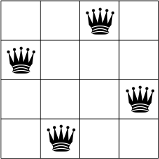
\includegraphics{4-queens.png}
            \caption{N-Queens}
            \label{fig:my_label}
        \end{figure}
    \end{itemize}
   
       
\end{document}